\section{Data}
The main input of the Article-Editor ranking algorithm is data generated by parsing all the edit histories of all the articles in Wikipedia category. We then only count editors which have made 5 or more edits to any article in any category, to eliminate page vandals. Also we discard all "Bots", software robots that programmatically edit Wikipedia. (When bots are included they rank as the fittest editors by far!).

We collected contribution data for articles in 12 categories (c.f. table \ref{tab:statistics} for summary statistics on the categories). In addition, we made 10 snapshots from the the earliest history to an equally increasing number of edits to account for the evolution over time of each category(see Figure \ref{fig:accumulative_snapshots} ).

\begin{table}
\begin{tabular}{lrrr}
\toprule
{} &  articles &  editors &   edits \\
\midrule
American male novelists               &      2460 &   9946 &  224783 \\
2013 films                            &      1896 &   5215 &  150956 \\
American women novelists              &      1936 &   5968 &  138716 \\
Nobel Peace Prize laureates           &       104 &   4165 &   91522 \\
Sexual acts                           &        93 &   2190 &   45901 \\
Economic theories                     &       212 &   1145 &   28658 \\
Feminist writers                      &       233 &   1357 &   25738 \\
Yoga                                  &       123 &    730 &   25315 \\
Military history of the US &       180 &    854 &   20172 \\
Counterculture festivals              &        66 &    578 &   10515 \\
Computability theory                  &        92 &    272 &    7117 \\
Bicycle parts                         &        70 &    210 &    4981 \\
\bottomrule
\end{tabular}
\caption{Size statistics of investigated Wikipedia categories sorted by total edits.}
\label{tab:statistics}
\end{table}

\begin{figure}[!t]
\centering
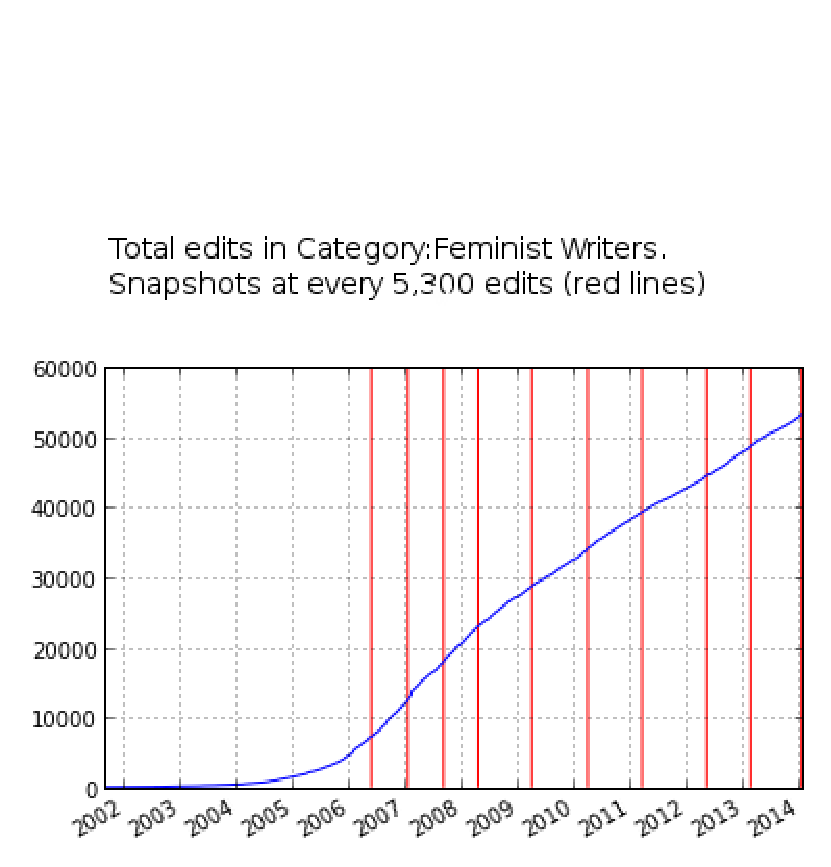
\includegraphics[width=0.9\columnwidth]{Figures/cumulative_snapshots_Feminist_Writers.eps}
\caption{Accumulative snapshots points for Category Feminist Writers. The snapshots is all the history {\it upto} the red line.}
\label{fig:accumulative_snapshots}
\end{figure}

For each snapshot, we constructed the matrix $\mathbf{M_{e,a}}$ of contributors versus edited articles, similar to the country versus products matrix of the Economics Domain. For each snapshot, the values in $\mathbf{M_{e,a}}$ are defined as the number of edits made by editor $e$ on article $a$ in the category occurring in the snapshot time. Note that the final snapshot represents the entire history of the category up to the present date.
  
The matrix $\mathbf{M_{e,a}}$ is a binary representation of $\mathbf{\hat{M}_{e,a}}$ where each nonzero entry is replaced with $1$. This represents if editors have touched which articles rather than how much they have touched each article. In the economics domain, the distinction of making a binary matrix out of the data is interpreted an alternative metric to GDP per capita, rather than GDP. Here we could also see the distinction as normalized editor fitness. The matrix $\mathbf{M_{e,a}}$ constitutes the basic input for implementing the biased Markov chain approach, $\mathbf{w^*}$.

In order to compare our results later, we draw exogenous variables for both editor and article ranks.

The exogenous metric we take for editors is {\it labour hours} a measure proposed by \cite{geiger2013}, denoted $v_e$ . 
This is calculated for each editor by taking contribution history upto the snapshot point, dividing into strings of {\it edit sessions}, edits that occur within 1 hour of the previous edit. Then we subtracting the first from last edit in each edit session, to get the length of the edit session. Lastly we sum edit sessions. 

For an exogenous measure of article quality, $ v_a$,  we use a group of 5 text analysis metrics performed on Wikipedia articles at the lastest time in the snapshot. The text metrics are mature relative to the age of Wikipedia \cite{stvilia} and used in suggesting tasks for editors \cite{wang}. These are (i) ratio of mark-up to readable text, (ii) number of headings, (iii) article length, (iv) citations per article length, and (v) outgoing intrawiki links. To reduce the dimensionality of these 5 metrics, we perform Principal Component Analysis, and accept the principal component. \cite{klein} Variance explained by the first principal component, was as high as 0.72 and lowest 0.50.
